\documentclass{article}
\usepackage{graphicx}
\usepackage{caption}
\usepackage{subcaption}

\author{Ruben Sharpe}
\title{Crime and the city:\\Spatial planning for crime reduction}
\date{\today}

\begin{document}
\maketitle

\begin{abstract}
 It is hypothesised that crime in a neighbourhood is correlated, albeit in a complex manner with the availability of public venues. Rather than hypothesising about causal relations, a machine learning approach is proposed in which high-crime, medium-crime and low-crime neighbourhoods are characterised by their public venues. These characterisations may serve as templates for good and bad practices in spatial planning.
 As a test case, the city of Toronto (Ontario, Canada) was characterised based on information about public venues, obtained from Foursquare, and the City government of Toronto Open Dataset on crime. 
 
 Neighbourhoods were clustered by similarity of their composition in terms of venues using K-means clustering.  
 Spatial information on crime was visualised in choropleth maps of Toronto. Visual comparison of neighbourhood clusters with crime maps shows the feasibility of the approach.
 
 Decision trees and support vector machines were trained to classify neighbourhoods as high-, medium- or low-crime. With such models, city planners may try to predict how modifications would impact the crime classification or, in other words, which modifications correlate with what crime level.
\end{abstract}

\tableofcontents



\section{Introduction}
It is intuitively clear that public venues, such as bars and restaurants, but also public service locations such as transport hubs or banks impact the wellbeing of local communities. However, it is not straightforward to predict whether this impact will be positive or negative. Bars and restaurants can enliven a neighbourhood and may contribute to greater safety because of an increased presence of people in the streets because potential witnesses deter crime. On the other hand, the presence of bars and restaurants is also correlated with alcohol abuse related crime. Similarly, there is a duality in the social impact for the presence of shops and banks. These may have a positive impact because of associated prosperity, but may also attract criminal activity at night because of reduced traffic compared to residential areas.\\

The complexity and the interrelatedness of these issues carries over to the complexity of city planning. The difficulty for city planners, moreover, is that they rarely get to design a neighbourhood from scratch. Typically, they have to deal with neighbourhoods with for the most part a fixed set of public facilities, and which may be suboptimal from a design point of view. The question for a city planner, therefore, is often: ``What would be, \emph{for a certain neighbourhood and given all its other attributes}, the impact of building (or removing) a shopping mall? Or a park? Or adding, or removing a bus stop?''\\

There is, of course, a lot of scientific literature on this topic but that is out of the scope of this project. This report is aimed at city planners and is intended to show the feasibility of machine learning as a tool for spatial planning.\\
Machine learning allows an automated approach to compare neighbourhoods both in terms of their public venues and in terms of social markers, such as crime rates. This provides city planners, apart from their professional expertise, with examples of good and bad practices that may help them in their decision making.\\
By way of example, the analysis in this report will look at the city of Toronto (Ontario, Canada). Crime rates will be used as the proxy for the wellbeing of communities, although other markers such as employment rate or health statistics could also be used.

\section{Data}
Location data, information about public venues and crime statistics will be used to classify neighbourhoods and map them with respect to the prevalence of crime. From this, generalised conclusions may be drawn with respect to the makeup of `high-crime' and `low-crime' neighbourhoods. 

\subsection{Location data}
Location data for the city of Toronto can be acquired by scraping postal codes, boroughs and neighbourhoods from Wikipedia.\footnote{https://en.wikipedia.org/wiki/List\_of\_postal\_codes\_of\_Canada:\_M} This data needs to be  enriched with the GPS coordinates of the respective neighbourhoods. These coordinates can be obtained from the internet in the form of a `.csv' file from the Coursera website for the Data Science Capstone.\footnote{https://cocl.us/Geospatial\_data} The enriched dataset consists of the postal codes, borough, and neighbourhood names and the neighbourhoods' latitude and longitude (Figure \ref{fig:enriched}).
\begin{figure}[ht]
 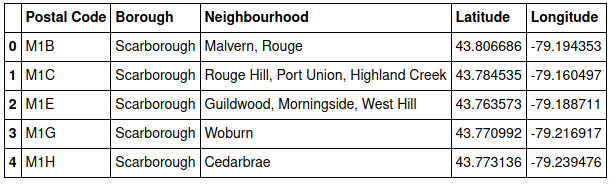
\includegraphics[width=\textwidth]{pics/enriched.png}
 \caption{Example of data enriched with coordinates.}
 \label{fig:enriched}
\end{figure}


\subsection{Public venues}
Foursquare is used to obtain information about the public venues, specifically their category, in each neighbourhood (Figure \ref{fig:venues}). For this purpose, the neighbourhood is arbitrarily defined as the area within a 1,500 m radius around a postal code's geographical centre. The top 10 most prevalent venues will be used to characterise the neighbourhood (Figure \ref{fig:grouped}).
\begin{figure}[ht]
 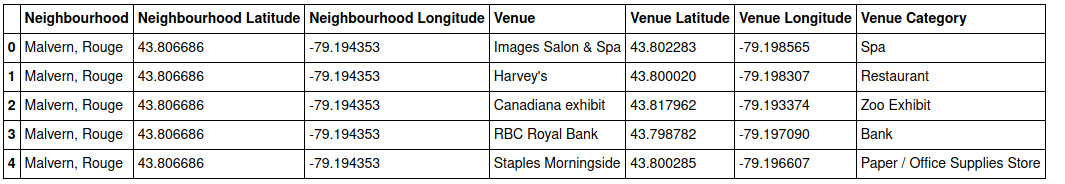
\includegraphics[width=\textwidth]{pics/venues.png}
 \caption{Example of which venue information can be obtained.}\label{fig:venues}
\end{figure}
\begin{figure}[ht]
 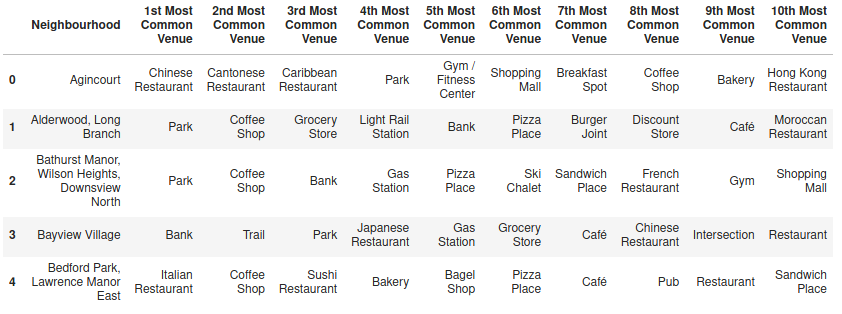
\includegraphics[width=\textwidth]{pics/grouped.png}
 \caption{Example of neighbourhoods with top 10 most prevalent venues.}\label{fig:grouped}
\end{figure}

\subsection{Crime data}
The city of Toronto provides a lot of open data related to the city.\footnote{https://www.toronto.ca/city-government/data-research-maps/open-data/} This data ranges from polls conducted by the government, to inventory lists of street furniture, to `bicycle count and locations' and is ever increasing. From this repository, a list of crime rates can be obtained.\footnote{https://open.toronto.ca/dataset/neighbourhood-crime-rates/} This list contains, for each neighbourhood the number of incidences of certain types of crime (Table \ref{tab:crime}). Population information from the 2016 census, included in the file, can be used to normalise crime rates relative to population size. Conveniently, the file also contains geographical information so that this information can be easily mapped. The crime categories that are accessible from the data files are given in Table \ref{tab:crime}.
\begin{table}[ht]
\centering
    \begin{tabular}{ll}
    \hline\hline
    Category & available data\\
    \hline
        Assault &  from 2014 -- 2019\\
        Auto Theft &  from 2014 -- 2019\\
        Breaking and Entering &  from 2014 -- 2019\\
        Homicide &  from 2014 -- 2019\\
        Robbery &  from 2014 -- 2019\\
        Theft &  from 2014 -- 2019\\
    \hline
    \end{tabular}
\caption{Crime data categories.}\label{tab:crime}
\end{table}



\section{Methodology}
\subsection{Exploration of crime information}
Crime information is available for six categories. This information may be visualised in choropleth maps (Figure \ref{fig:nbhcrime}). Since there are six crime categories, a neighbourhood classification in `high-', `medium-' or `low-crime' must either relate to one of the six categories, or a new crime index must be constructed. 
\begin{figure}[ht]
     \centering
     \begin{subfigure}[b]{0.47\textwidth}
         \centering
         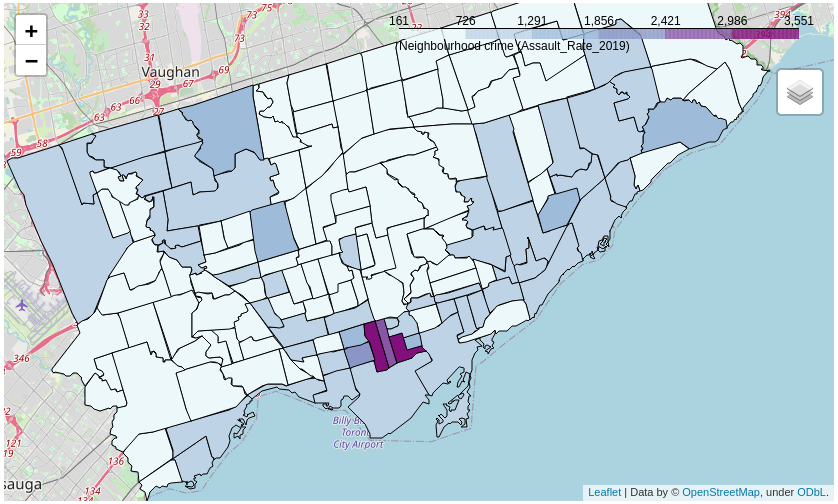
\includegraphics[width=\textwidth]{pics/assault2}
         \caption{Assault}
     \end{subfigure}
     \hfill
     \begin{subfigure}[b]{0.47\textwidth}
         \centering
         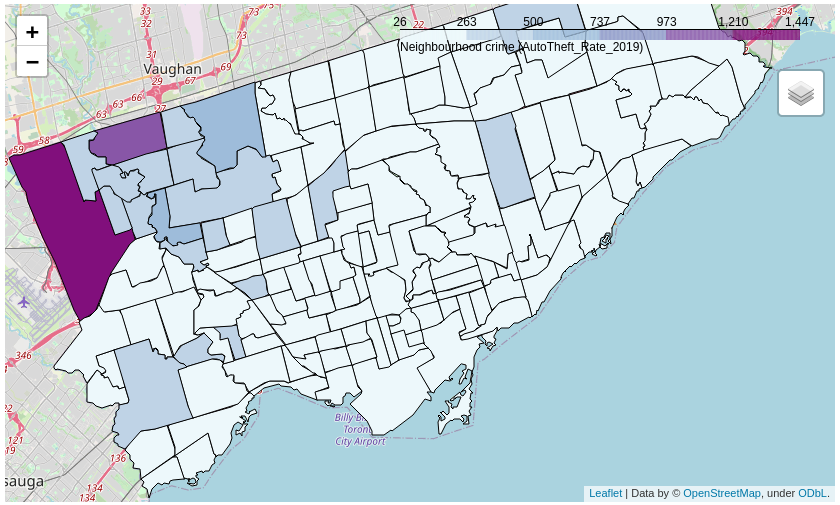
\includegraphics[width=\textwidth]{pics/auto}
         \caption{Auto theft}
     \end{subfigure}
     \begin{subfigure}[b]{0.47\textwidth}
         \centering
         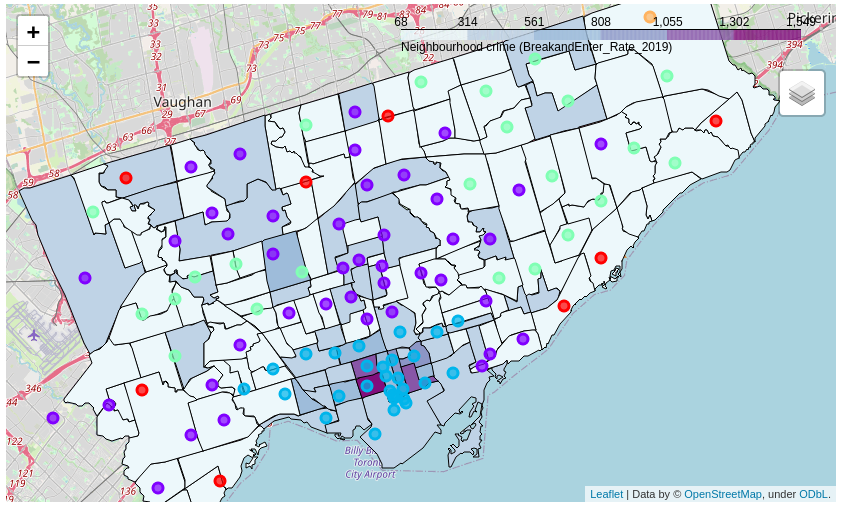
\includegraphics[width=\textwidth]{pics/breakenter}
         \caption{Breaking and entering}
     \end{subfigure}
     \hfill
     \begin{subfigure}[b]{0.47\textwidth}
         \centering
         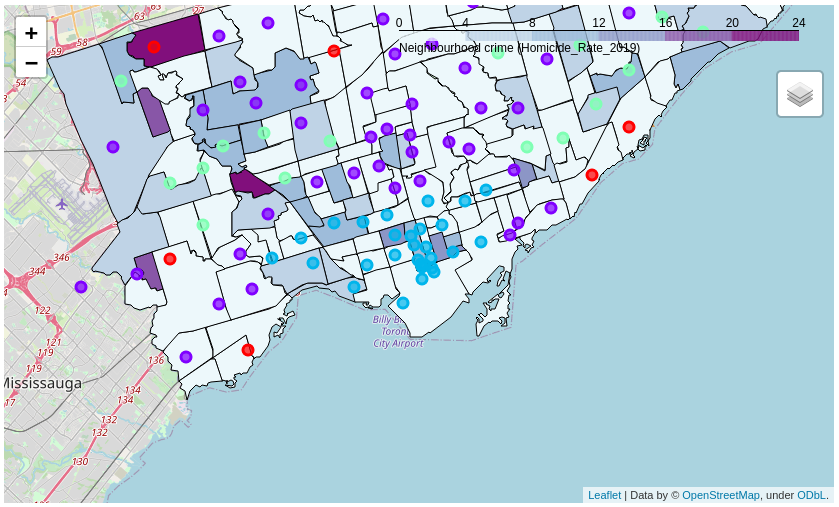
\includegraphics[width=\textwidth]{pics/homicide}
         \caption{Homicide}
     \end{subfigure}
     \begin{subfigure}[b]{0.47\textwidth}
         \centering
         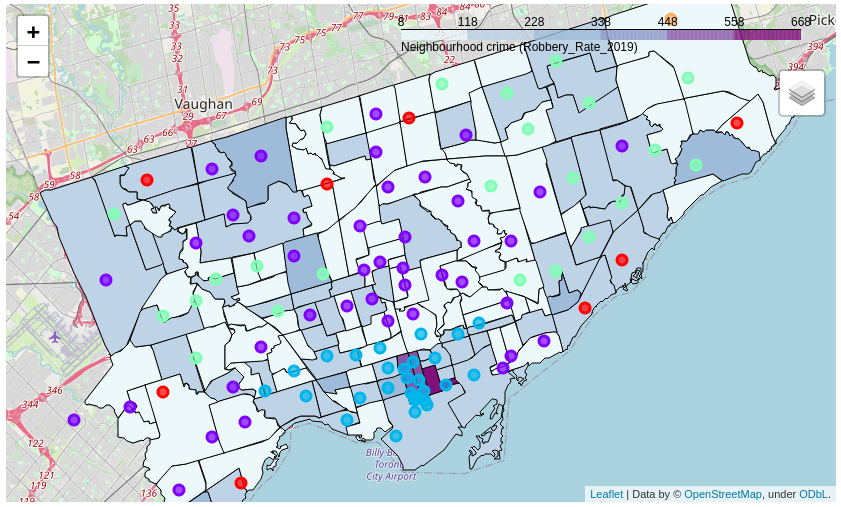
\includegraphics[width=\textwidth]{pics/robbery}
         \caption{Robbery}
     \end{subfigure}
     \hfill
     \begin{subfigure}[b]{0.47\textwidth}
         \centering
         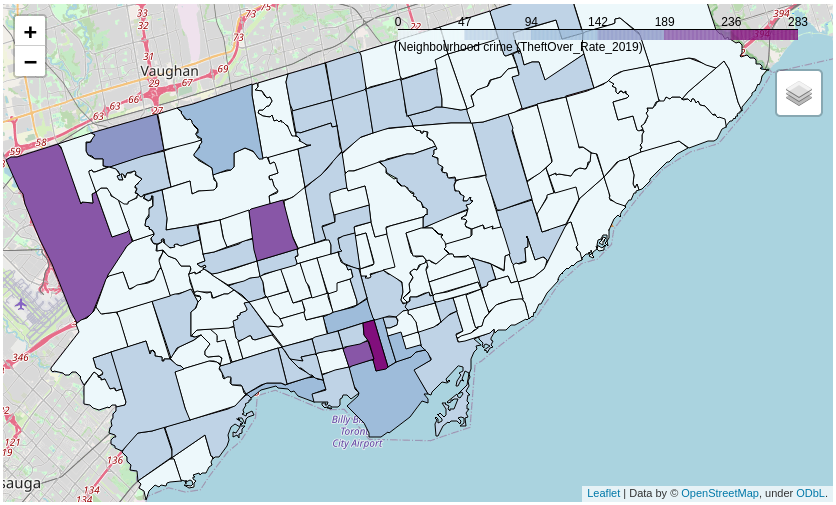
\includegraphics[width=\textwidth]{pics/theftover}
         \caption{Theft other}
     \end{subfigure}
        \caption{The six crime categories and their spatial distribution (2019 crime rates).}
        \label{fig:nbhcrime}
\end{figure}

In order to create a crime index, each crime category is first normalised with respect to the maximum number of occurrences across all neighbourhoods. Then these indices are summed over all the six crime categories and normalised again with respect to the maximum of this new `overall' category. The index can be interpreted as follows: an index of `1' means that the neighbourhood has scored, on average, the worst in all crime categories, whereas an index of `0' means that there have been no incidences of crime in any of the categories in that neighbourhood. Therefore, areas with indices up to 0.3 are labeled `low-crime', areas with indices between 0.3 and 0.7 are labeled `medium-crime' and areas with indices higher than 0.7 are labeled `high-crime'.

For convenience, the 2019 crime rate for each crime category is used. These are already represented as incidents per 100.000 population and therefore the population size of each neighbourhood does not need to be taken into account.

By visually comparing the crime index choropleth with the spatial distribution of the neighbourhoods in the venue dataset, the latter can be manually labeled with respect to the crime index (Figure \ref{fig:manual}). 
\begin{figure}[ht]
    \begin{subfigure}[b]{0.47\textwidth}
        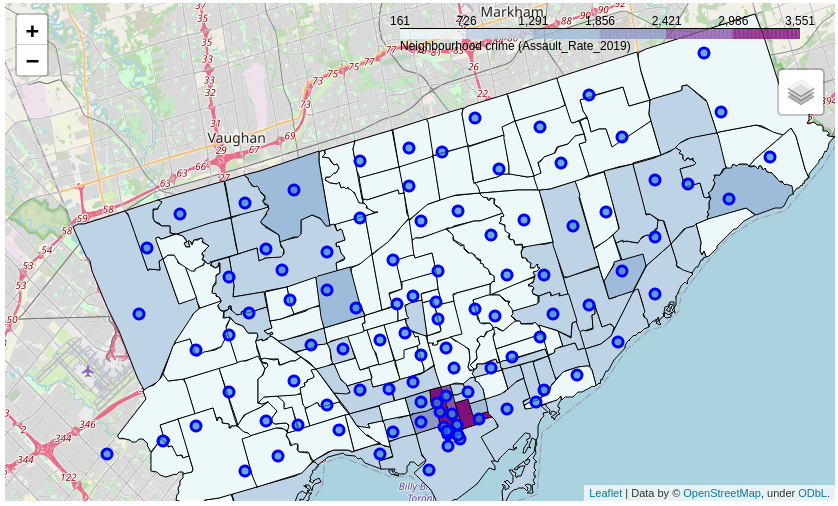
\includegraphics[width=\textwidth]{pics/manual.png}
        \caption{}
    \end{subfigure}\hfill
    \begin{subfigure}[b]{0.47\textwidth}
        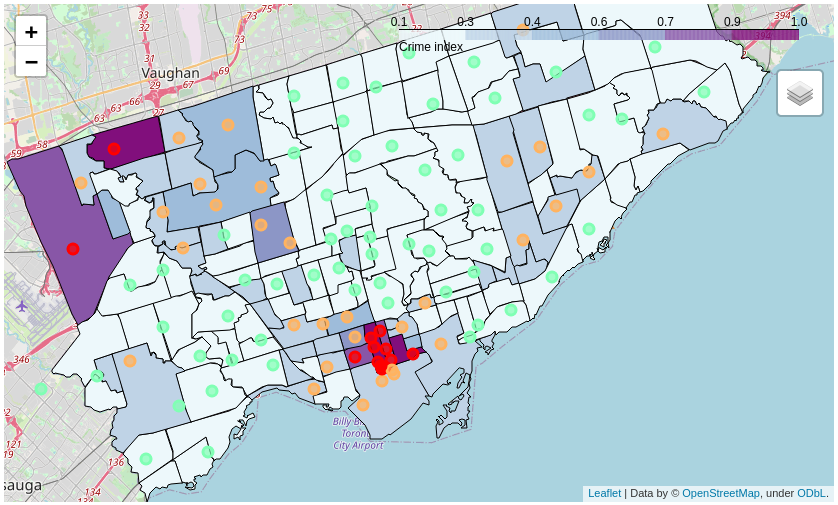
\includegraphics[width=\textwidth]{pics/manual2.png}
        \caption{}
    \end{subfigure}
    \caption{Spatial correlation of crime with neighbourhood information (a). Neighbourhoods that lie on purple areas may be manually labeled 'high-crime' (red dots), neighbourhoods on blue areas `medium-crime' (yellow dots) and neighbourhoods on light blue areas `low-crime' (light blue dots)(b).}\label{fig:manual}
\end{figure}



\subsection{Machine learning}
\subsubsection{Unsupervised clustering of neighbourhoods and visual correlation with crime}
Similarity of neighbourhoods with respect to their public venues, as well as the spatial distribution of similar neighbourhoods is explored using K-means clustering. A qualitative correlation between the neighbourhood clusters and crime can be obtained by visual inspection of crime and cluster maps. Different clusters that spatially correlate with different crime indices indicate a correlation between neighbourhood composition and crime. The more dissimilar two clusters are, the more intuitive it is to make future predictions for a given neighourhood composition. 

An idea of the intra- and inter-cluster similarities can be obtained by inspecting the output of the clustering algorithm for increasing numbers of clusters. From this, it can be observed which clusters break up first and which stay intact.  Clusters that break off from larger clusters are siblings and share some inter-cluster similarity. Clusters that resist breaking up, indicate high intra-cluster cohesion (i.e. greater internal similarity). Because the most distinct clusters are the most intuitively useful, it is best to focus on non-sibling clusters with large intra-cluster similarity.

\subsubsection{Modelling}
Whereas K-means clustering may be used to qualitatively classify clusters of varying venue composition by crime index, it is not necessarily obvious how changes in the neighbourhood composition (of a specific neighbourhood) cause its classification to change. In other words, it is from K-means clustering not obvious which changes would cause a certain neighbourhood to become more or less similar to neighbourhoods with a more desirable crime rating. For this reason, a decision tree model will be built. Such a model will allow parsing of changes to a neighbourhood's composition and a prediction of the new crime rating. Decision trees are also very intuitive and their explicit structure facilitates the upfront estimation of which changes the outcome will be most sensitive to. For reasons of comparison, however, a support vector machine classifier will also be built.

\section{Results}
\subsection{Visual inspection}
The K-means algorithm has been run to create 3, 4 , 5 and 7 clusters of neighbourhoods (Figure \ref{fig:nbhclusters}). From this, it can be seen that there are basically two large clusters with high inter-cluster similarity: one centred around the harbour and one broad band from east to west. Increasing the number of clusters causes smaller break-away clusters, mostly from the second (`broad band') cluster. This indicates that for higher numbers of clusters, the main division will still be between the `harbour cluster' and the other clusters that share some commonality with the original `broad band' cluster. The nature of the dissimilarity that causes this division, however, is not intuitively clear from inspection of the most prevalent venues in each group (`harbour cluster' versus `broad band offspring clusters') (Figure \ref{fig:composition}).
\begin{figure}[ht]
     \centering
     \begin{subfigure}[b]{0.47\textwidth}
         \centering
         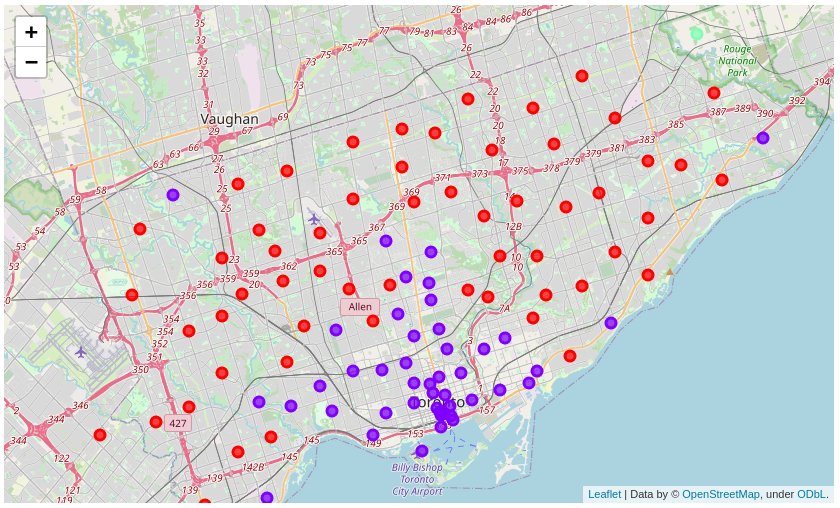
\includegraphics[width=\textwidth]{pics/clusters3}
         \caption{Three clusters}
     \end{subfigure}
     \hfill
     \begin{subfigure}[b]{0.47\textwidth}
         \centering
         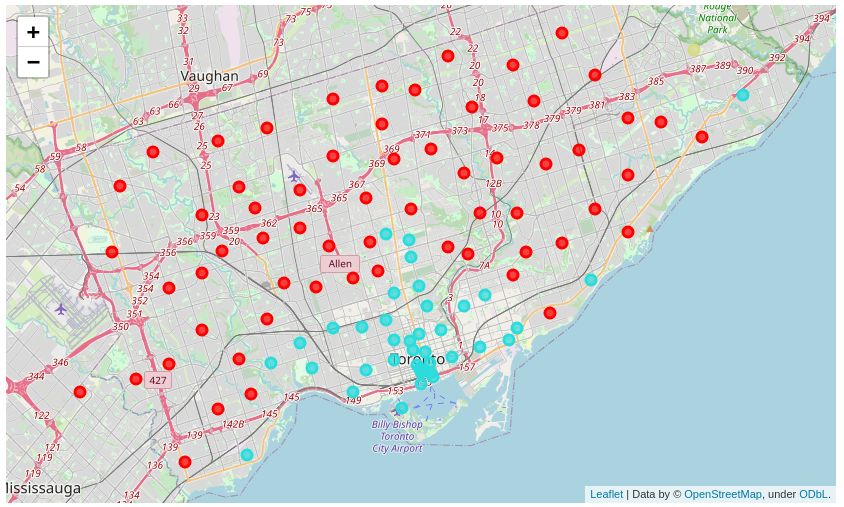
\includegraphics[width=\textwidth]{pics/clusters4}
         \caption{Four clusters}
     \end{subfigure}
     \begin{subfigure}[b]{0.47\textwidth}
         \centering
         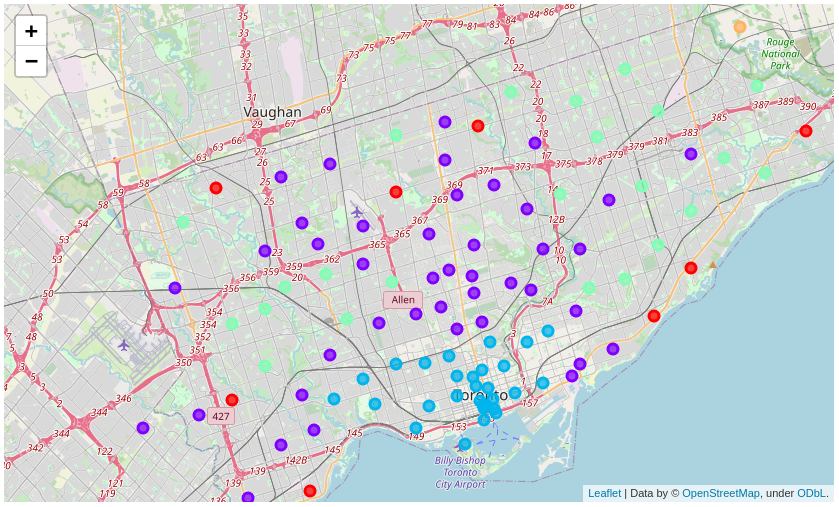
\includegraphics[width=\textwidth]{pics/clusters5}
         \caption{Five clusters}
     \end{subfigure}\hfill
     \begin{subfigure}[b]{0.47\textwidth}
         \centering
         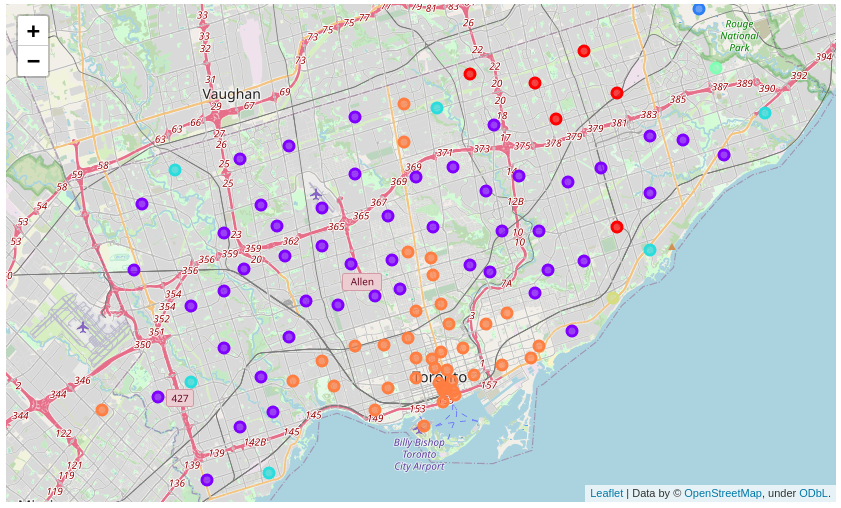
\includegraphics[width=\textwidth]{pics/clusters7}
         \caption{Seven clusters}
     \end{subfigure}
     \caption{Different distributions of three, four, five and seven clusters. Note that there are basically two stable clusters, concentrically oriented around the harbour. Increasing the number of clusters only causes small split-offs.}
        \label{fig:nbhclusters}
\end{figure}
\begin{figure}[ht]
     \centering
        \begin{subfigure}[b]{\textwidth}
            \centering
            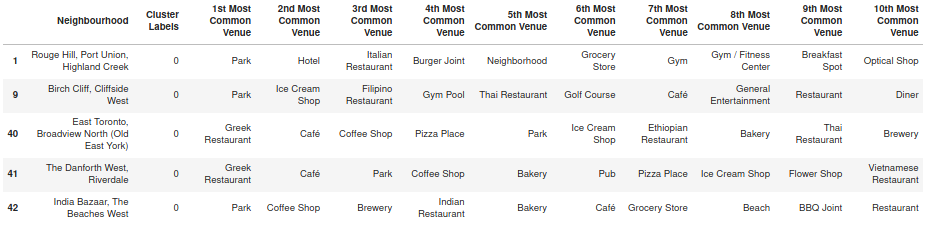
\includegraphics[width=\textwidth]{pics/composition_0}
            \caption{Venue composition of first five neighbourhoods in the `harbour' cluster.}
        \end{subfigure}
        \begin{subfigure}[b]{\textwidth}
            \centering
            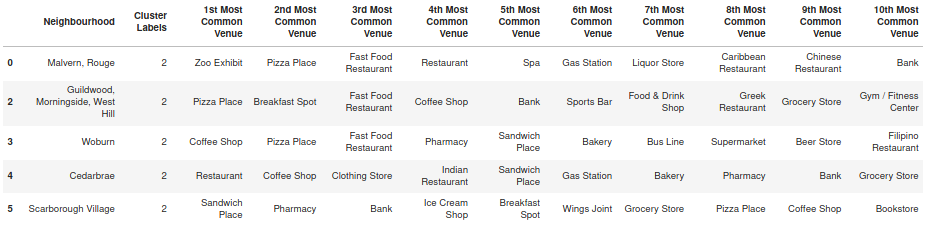
\includegraphics[width=\textwidth]{pics/composition_2}
            \caption{Venue composition of the first five neighbourhoods in the `broad band' cluster.}
        \end{subfigure}
        \caption{Compositions of the most stable clusters. Note that although these are stable and therefore very dissimilar, the dissimilarity is not intuitively obvious.}
        \label{fig:composition}
\end{figure}

Spatially, the clusters correlate somewhat with the crime map, insofar that a relatively high crime index is found in the neighbourhoods around the harbour and in the North-West corner of Toronto. This agrees reasonably well with the spatial distribution of the harbour cluster, which is marked with red dots in Figure \ref{fig:clustercrime}. A significant amount of neighbourhoods belonging to the harbour cluster, moreover are found in low-crime areas. The cluster distribution, furthermore, does not clearly discriminate between medium and low crime indices which both are equally well covered by the broad band cluster, which is marked with blue dots in Figure \ref{fig:clustercrime}.
\begin{figure}[ht]
\centering
 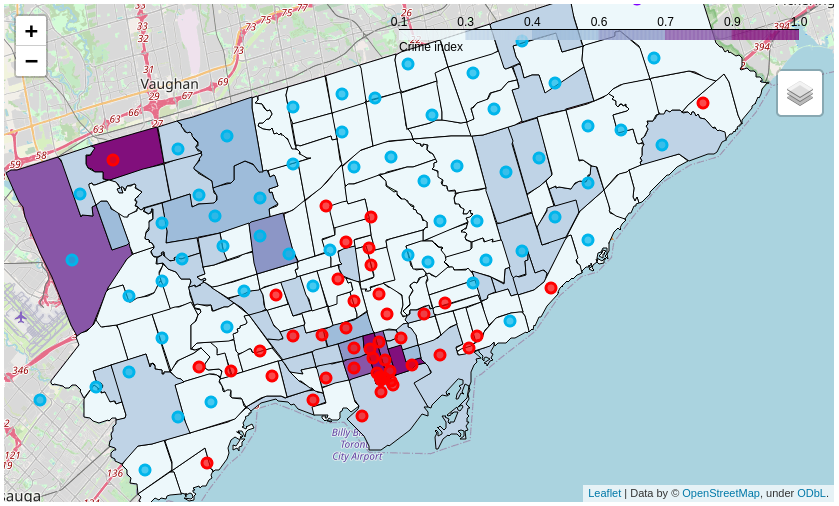
\includegraphics[width=\textwidth]{pics/clustercrime.png}
 \caption{Spatial distribution of crime and of clusters with a similar public venue composition.}\label{fig:clustercrime}
\end{figure}

\subsection{Decision tree and SVM}
A decision tree is built with an overall test accuracy of 0.76. This indicates that 76\% of a test set has been correctly predicted. However, the number of high-crime neighbourhoods is far smaller than the number of medium- and low-crime neighbourhoods so that a high overall accuracy can still be obtained with a high number of mislabelling of the high-crime neighbourhoods. In fact, the Jaccard accuracy for high-crime is only 0.25 while the Jaccard accuracy for medium-crime is 0.56 and that for low-crime is 0.77 (Table \ref{tab:accuracy}). This is also clearly visible when the decision tree is trained on the full set of neighbourhoods (with an overall training accuracy of 0.92) and the newly predicted labels are plotted on the crime index choropleth (Figure \ref{fig:predicted}).
\begin{figure}[ht]
\centering
    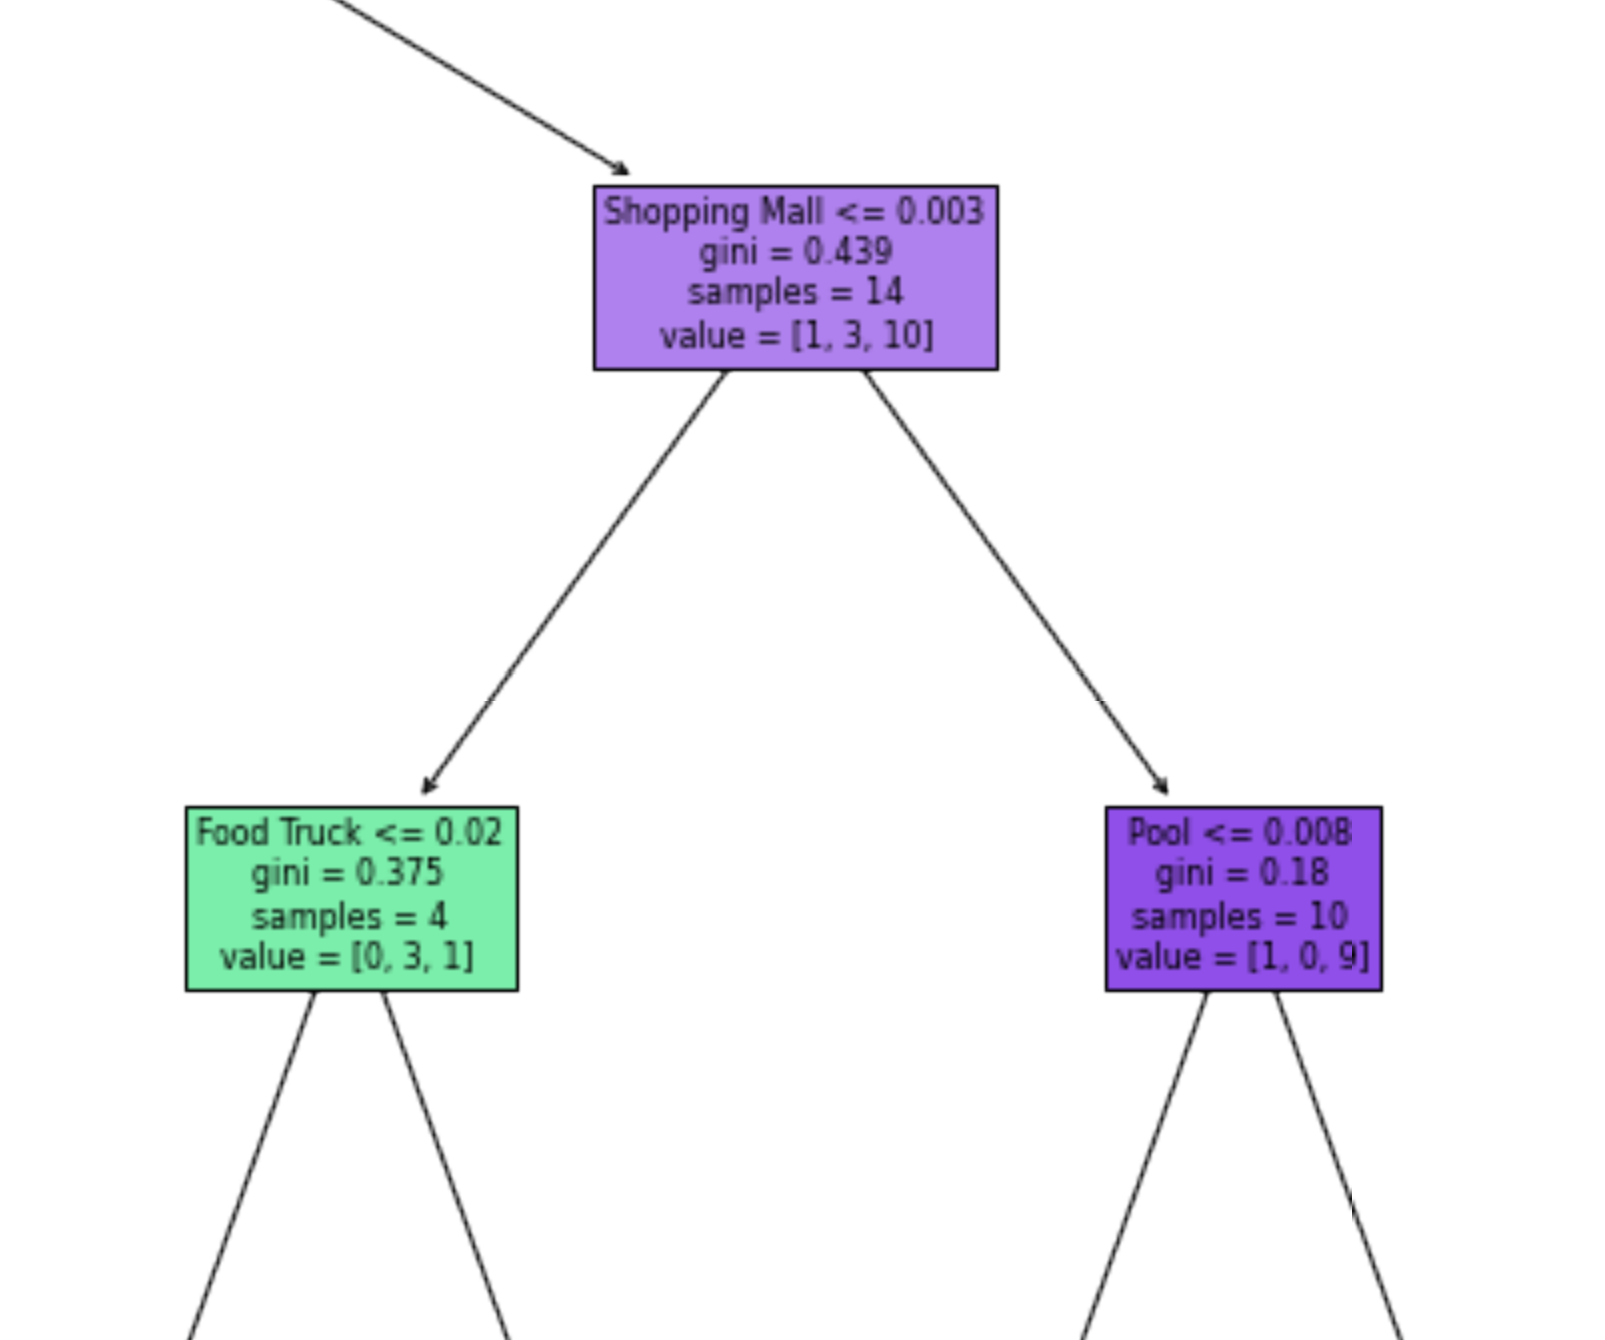
\includegraphics[width=0.6\textwidth]{pics/detail.png}
    \caption{Detail of the decision tree illustrating the explicit nature of the decisions that lead to a certain classification. Decision trees may therefore be used to predict to which tweaks the classification is particularly sensitive.}\label{fig:tree}
\end{figure}
\begin{table}
\centering
\begin{tabular}{lll}
 \hline\hline
 Accuracy type & Decision tree & SVM\\
 \hline
 Overall & 0.76 & 0.57\\
 Jaccard `high' & 0.25 & 0.0\\
 Jaccard `medium' & 0.56 & 0.29\\
 Jaccard `low' & 0.77 & 0.59\\
 \hline
\end{tabular}\caption{Accuracy of the decision tree predictions (on a test set).}\label{tab:accuracy}
\end{table}
\begin{figure}[ht]
\centering
 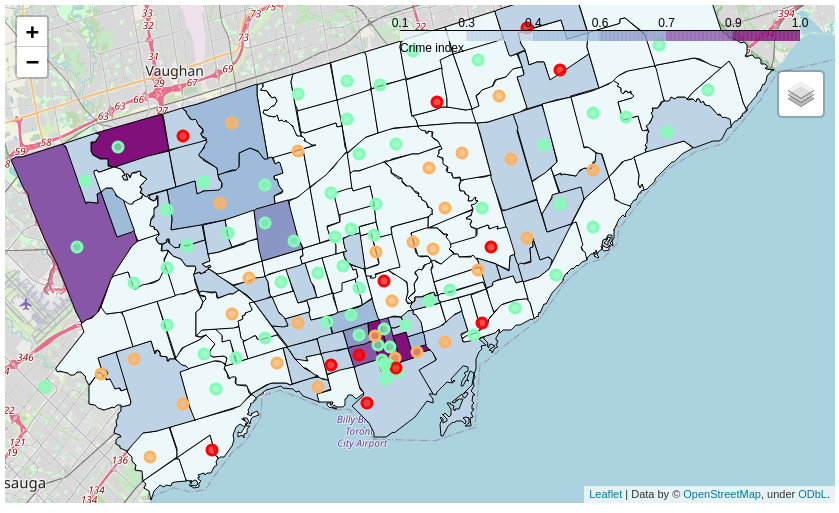
\includegraphics[width=\textwidth]{pics/prediction.png}
 \caption{Graphical representation of the correlation between the predicted (via decision tree) and observed crime indices. Mislabelling of high-crime neighbourhoods is most frequent (red dots), whereas low crime neighbourhoods were most accurately predicted (light blue dots).}\label{fig:predicted}
\end{figure} 

For reasons of comparison, also a support vector machine (SVM) has been trained. The overall test accuracy of the SVM was 0.57, which is significantly lower than that of the decision tree. The Jaccard scores for high-, medium- and low-crime were 0(!), 0.29 and 0.59 respectively. Again, those are clearly worse than the decision tree predictions.

\section{Discussion}
\subsection{Correlating neighbourhood composition with high-crime areas}
By visual inspection of similar neighbourhoods and crime data, a correlation between neighbourhood composition and crime rate may be inferred (Figure \ref{fig:nbhclusters}). The cluster with the most internal cohesion (i.e. which is most resistant to breaking up) is situated concurrend with high-crime neighbourhoods and therefore its composition may be qualitatively interpreted as indicative of higher occurrences of crime.

Although the cluster that correlates most strongly with high-crime areas is clearly distinct from the other clusters that correlate with medium- and low-crime areas, the distinction is not intuitive (Figure \ref{fig:composition}). Medium- and low-crime areas correlate less strongly with neighbourhood clusters than high-crime areas. Moreover, any such clusters that do correlate with medium- and low-crime areas are siblings, i.e. they are more similar to each other than they are to the high-crime cluster. It may be expected that these are therefore even harder to distinguish between each other.

The reason that clusters are indistinct to a human interpreter is that clustering was performed on relatively similar data sets: By focussing on the top 10 most prevelant venues a bias is introduced toward the venue types of which there are relatively many. For any neighbourhood it is more likely to have, e.g. multiple restaurants than to have multiple airports. Therefore, many neighbourhoods are likely to have restaurants in their top 10, simply because these are relatively common. Conversely, an airport is not likely to feature in any neighbourhood's top 10 even though an airport is likely to have a big impact on a neighbourhood's wellbeing and crime rating.

All this means that a lot of professional expertise is required in order to use the current cluster characterisations to predict which manipulations of the neighbourhood composition might be favourable.

\subsection{Correlating neighbourhood composition with medium- and low-crime areas}
Whereas K-means clustering and visual inspection favour a qualitative correlation between neighbourhood composition and high-crime areas, the opposite is true for decision trees and SVMs. Because the vast majority of the neighbourhoods in Toronto can be classified as either low-, or medium-crime, the algorithm is skewed toward those. Specifically low crime neighbourhoods can be predicted with relatively high accuracy but this accuracy quickly deteriorates toward high-crime (Table \ref{tab:accuracy}). This is, however, not necessarily a problem for city planners. Since they most likely aim to improve a neighbourhood, they would be most  interested in how to increase its similarity with low-crime areas (starting from an already known higher crime composition). 

Compared to SVMs, decision trees have been found to be the most accurate. Because of their explicit decision structure they are also the most helpful for planning interventions.

\section{Conclusion}
Machine learning, specifically K-means clustering, decision trees and SVMs have been explored for their feasibility to support city planners to reduce crime. It has been shown that this is indeed the case, albeit with limitations.

The useability of K-means clustering relies on the ability of a human interpreter to make useful distinctions. In this study, the meaningful differences were found to be small. This may be due to a lack of distinctive features in the top 10 most prevalent venues for each neighbourhood. For further study it is advisable to look deeper into the dataset for features that may be less prevalent but more distinctive and more predictive.

Decision trees, although overall relatively accurate, are heavily skewed in favour of the most abundant category in the training set. In this study, the training set was a random sample of the actual Toronto neighbourhoods and therefore reflected the city's low-crime bias. For future study it may be interesting to selectively sample for a more proportional training set.

Overall it may be concluded that machine learning may be a powerful tool in a city planner's toolkit. For now, however, a solid professional expertise is still required.
 
\end{document}
